\documentclass[11pt,a4paper]{jsarticle}                    % fir platex
%\documentclass[11pt,a4paper,uplatex]{ujreport} 	% for uplatex
%
\usepackage{amsmath,amssymb}
\usepackage{bm}
\usepackage{graphicx}
\usepackage{ascmac}
\usepackage{float}
%
\setlength{\textheight}{40\baselineskip}
\addtolength{\textheight}{\topskip}
\setlength{\voffset}{-0.2in}
\setlength{\topmargin}{0pt}
\setlength{\headheight}{0pt}
\setlength{\headsep}{0pt}

\setlength{\textwidth}{\paperwidth}     % ひとまず紙面を本文領域に
\setlength{\oddsidemargin}{-5.4truemm}  % 左の余白を20mm(=1inch-5.4mm)に
\setlength{\evensidemargin}{-5.4truemm} % 
\addtolength{\textwidth}{-40truemm}     % 右の余白も20mmに
%
\title{脳波解析のための数学シリーズ\\
統計編}
\author{後藤 優仁}
\date{\today}
\begin{document}
\maketitle

\newpage
%
%
\tableofcontents
\newpage
\section{はじめに}
 統計処理とは, 実際に実験やアンケートを通して集めたデータを解釈する際に必要になる処理です. 論文を読むためにも必須, というか一番大事な項目なので頑張りましょう. analysisの様々な処理を行った結果,実験で計測した脳波を何らかの形で解釈しやすいようなデータに変形する事が出来ました.つまり解析をしました.次に必要なのは,この解析で得られたデータを解釈する行程です.ここで必要になるのが統計的な処理ですね.個人的には楽しくないですが,仕方ないのでやっていきましょう.\\
  また,結局脳の計算をモデル化しようとか発展的な議論をしていこうと思った時にはここら辺が非常に重要になってきます.先に勉強しておくとだいぶ後が楽だと思いますが,何に役立つのか分からないとモチベは上がらないし勉強できないのは自分も痛いほど分かるので,逆に先にadvanced.pdfとかでチラ見してくるのも良いかもしれませんね.\\
  特に,今はまだ追加できていませんがベイズ統計は勉強しておくべきです.勉強するだけで色々と広がっていきます.本当に.
 
 \newpage
 
 
\section{確率分布}
\subsection{確率分布と確率密度関数}
確率とは, 起こりうる全体の事象のうち, ある事象がどれくらいの割合で起こるのかを表します. 確率分布とは, 起こりうる事象それぞれの確率がどのような分布をしているかです. \\
確率密度関数とは, 実際に確率分布をプロット(横軸に事象, 縦軸に確率)した際に現れる分布の形を表現する関数の事です. 場合によっては事象は離散分布になったりするため,その場合はこの分布を連続と見立てて確率密度関数が定義されます.\\

\subsection{一様分布/ベルヌーイ分布/2項分布/ポアソン分布}
まずは簡単な分布から見て, 徐々に複雑なものを見ていきます. 今回は脳の数学であまり使わない気がするやつらはまとめて雑に確認します.\\
\subsubsection{一様分布}
例えばサイコロを振った時に出る目の確立分布を考えると, 当然6つの事象それぞれがすべて$\frac{1}{6}$で表せるため, プロットすると以下のようになります.\\
\begin{figure}[H]
\label{im:uniform}
  \centering
  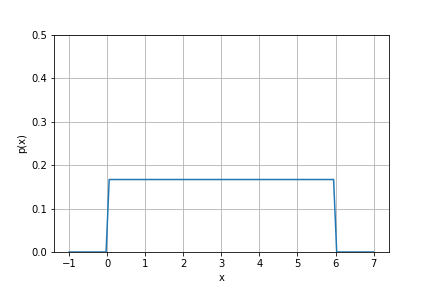
\includegraphics[width=120mm,bb=0 0 432 288]{../figures/uniform.png}
  \caption{サイコロの確立分布(一様分布)}
\end{figure}

一様分布は確率密度関数を定義するまでもないのですが, 勉強のためにあえてやるとすると以下のようになります. まずさいころの例だとそれぞれの目が出てくる確率はこうですね.

\begin{eqnarray}
\label{eq:uniform}
f(x) = \frac{1}{6} (1 \leq X \leq 6)
\end{eqnarray}

定義域が0から6で, いずれの点においても$\frac{1}{6}$の確立で目がでるよってことですね. 簡単です. また確率を考える際, 式(\ref{eq:uniform})のように左辺の$(x)$と右辺定義域内にいる$(X)$で使い分けがなされます. $X$は確率変数を表し, 実際の値は取りません. 観測されて確定した時には$x$として表現されます. 今回の$X$と$x$の関係は

\begin{eqnarray}
X = [x_1, x_2, x_3, x_4, x_5, x_6]
\end{eqnarray}
のような感じです. \\
\\
より一般には離散一様分布に従う変数の確率関数は,Nを変数が取りうる値(さいころの目=6)として,

\begin{eqnarray}
P(X=x) = \frac{1}{N} \qquad (x=1,2,...,N)
\end{eqnarray}
となります.これはさすがに良いですよね.次.\\
離散一様分布の期待値と分散は以下です.\\

\begin{eqnarray}
\begin{split}
\mathbb{E}(X) &= \sum_{k=1}^N{kP(X=k)}\\
&=\sum_{k=1}^N{k\frac{1}{N}}\\
&= \frac{(1+N)N}{2}\frac{1}{N}\\
&= \frac{1+N}{2}
\end{split}
\end{eqnarray}

\begin{eqnarray}
\begin{split}
\mathbb{V}(X) &= \mathbb{E}(X^2) - \mathbb{E}(X)^2\\
&= \sum_{k=1}^N k^2 \frac{1}{N} - {(\frac{1+N}{2})}^2\\
&= \frac{1}{N}N\frac{(N+1)(2N+1)}{6}-\frac{(N+1)^2}{4}\\
&= \frac{N^2-1}{12}
\end{split}
\end{eqnarray}
\\
一見複雑?な気もするかもしれませんが,普通に計算してみればわかるとおもいます.ほら,「1から100までの数の和は?」みたいな問題って工夫して暗算出来ましたよね?どうやるんでしたっけ.\\
\\
連続一様分布については確率密度関数は以下のようになります.

\begin{eqnarray}
f(x) = 
\left\{
    \begin{array}{l}
      \frac{1}{b-a} \qquad \qquad  (a \leq X \leq b) \\
      0  \qquad \qquad \qquad(otherwise)
    \end{array}
  \right.
\end{eqnarray}

これは面積で考えると分かりやすいかも.確率密度関数は積分すると1にならないといけません.b-aは定義域なので,つまり面積でいうところの横の長さです.縦の長さはそれぞれの値が観測される確率,つまり$f(x)$ですよね?\\
そう,なので定義の$f(x)$を定義域で積分すると1になります.当たり前の事なのですが,確率密度関数の考え方にいまいち慣れていない人ように丁寧に言いました.以下はこのような話は省略します.\\
とにかく,積分すると1になるのが確率密度関数です.


平均$\mathbb{E}(X)$及び分散$\mathbb{V}(X)$は

\begin{eqnarray}
\mathbb{E}(X) = \frac{a+b}{2}\\
\mathbb{V}(X) = \frac{(b-a)^2}{12}
\end{eqnarray}

一応,期待値くらいは証明もしておきます.でもまあ簡単です.

\begin{eqnarray}
\begin{split}
\mathbb{E}(X)  &= \int_{-\infty}^{\infty} xf(x) dx \\
&= \int_{-\infty}^{a} xf(x) dx + \int_{a}^{b} xf(x) dx + \int_{b}^{\infty} xf(x) dx \\
&= 0 + \int_{a}^{b} x\frac{1}{b-a} dx + 0\\
&= \frac{1}{b-a}\left[\frac{x^2}{2}\right]_a^b\\
& = \frac{b-a}{2}
\end{split}
\end{eqnarray}

\subsubsection{ベルヌーイ分布}
ベルヌーイ分布は, 1か0かです. ある事が起きるか起きないか, 成功するかしないかなどの2値分類ですね. 超簡単です!!\\

\begin{figure}[H]
\label{im:bernoulli}
  \centering
  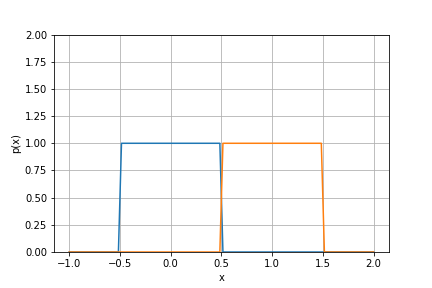
\includegraphics[width=120mm,bb=0 0 432 288]{../figures/bernoulli.png}
  \caption{ベルヌーイ分布}
\end{figure}
今回は1:1の図になっていますが, もちろん1:5くらいの割合になる事もあります. たとえばサイコロで1が出るか出ないかとか. 以上.\\
\\
関数はこんな感じかな
\begin{eqnarray}
f(x)=
  \left\{
    \begin{array}{l}
      p \qquad \qquad \qquad (x = 1) \\
      q(=1-p)  \qquad (x=0)
    \end{array}
  \right.
\end{eqnarray}

平均$\mathbb{E}(X)$及び分散$\mathbb{V}(X)$は

\begin{eqnarray}
\mathbb{E}(X) = p\\
\mathbb{V}(X) = pq
\end{eqnarray}

です. 興味ないので証明とかやりません. 僕も知らない.
\subsubsection{2項分布}
2項分布は「同じことを何回も繰り返した時, ある事柄が何回おこるか」の確立分布です. こいつは式を見れば早いですね.

\begin{eqnarray}
\label{eq:binomial}
f(x) = {}_n\mathrm{C}_x p^x(1-p)^{n-x}
\end{eqnarray}

式(\ref{eq:binomial})の右辺左側にある${}_n\mathrm{C}_x p^x$は, 確率pで起こる事象Aが, 全体nのうちx回でたという意味で, 右側の$(1-p)^{n-x}$は確率(1-p)で, Aが起きなかった回数が(n-x)回出たという意味です.\\
これらを掛け合わせているので, 何回当たって何回外れたかを表す式ですね.

\begin{figure}[H]
\label{im:bernoulli}
  \centering
  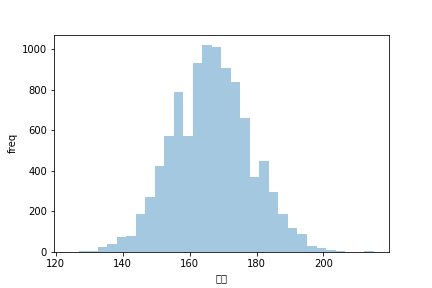
\includegraphics[width=120mm,bb=0 0 432 288]{../figures/binomial.png}
  \caption{ベルヌーイ分布}
\end{figure}

平均$\mathbb{E}(X)$及び分散$\mathbb{V}(X)$は

\begin{eqnarray}
\mathbb{E}(X) = np\\
\mathbb{V}(X) = np(1-p)
\end{eqnarray}

です. 興味ないので証明とかやりません. 僕も知らない.

\subsubsection{ポアソン分布}
ポアソン分布は「稀な事象が一定時間内にどれくらい起きるか」です.\\
たとえば, ある月にある地域で起きた交通死亡事故の件数とかです. 修羅の国やグンマ―, あるいは名古屋でもない限り, 普通は0か多くて2件とかですよね.\\
\\
確率密度関数は以下です.
\begin{eqnarray}
f(x) = \frac{\lambda^x}{x!}e^{-\lambda}
\end{eqnarray}

平均$\mathbb{E}(X)$及び分散$\mathbb{V}(X)$は

\begin{eqnarray}
\mathbb{E}(X) = \lambda\\
\mathbb{V}(X) = \lambda
\end{eqnarray}

です. こいつの場合, 平均も分散も同じ定数$\lambda$なので, こいつの値だけで形が決まります. $\lambda$がどんな値なのか, どうやって決まるのかは知りません. 使う事があれば足します.\\

\begin{figure}[H]
\label{im:poisson}
  \centering
  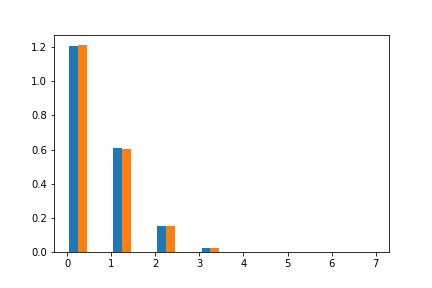
\includegraphics[width=120mm,bb=0 0 432 288]{../figures/poisson.png}
  \caption{ポアソン分布}
\end{figure}

\subsection{正規分布}
\subsubsection{正規分布とは}
さて本題です. 数ある確率分布の中でも抜きんでて重要な分布, 正規分布, またの名をガウス分布です. 世の中の多くの事象がこの分布に従っていて, また従っていると仮定して統計的処理がされています. 今後の統計学の基礎になるのでしっかり理解しましょう.\\
\\
正規分布は, 平均$\mathbb{E}(X)$が母集団の平均$μ$と等しく, 分散$\mathbb{V}(X)$も母集団の分散$\sigma ^2$と等しくなる分布で, 確率密度関数は以下になります.

\begin{eqnarray}
\label{eq:normal}
f(x) = \frac{1}{\sqrt{2\pi\sigma^2}}e^{-\frac{(x-\mu)^2}{2\sigma^2}}
\end{eqnarray}

いや, うん. 分かります. やばそうですよね. \\
ただまぁ, なんでこんな殺意高めな式になるのかは正規分布のグラフを見れば理解できます. 母集団の平均が50, 標準偏差20の正規分布だとこうなります.

\begin{figure}[H]
\label{im:normal}
  \centering
  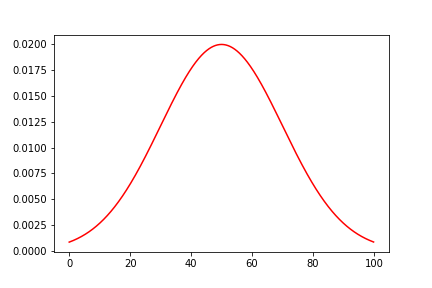
\includegraphics[width=120mm,bb=0 0 432 288]{../figures/normal.png}
  \caption{正規分布}
\end{figure}

定義通り, 確率変数の平均も50, 分散も400(20の二乗)になっていますね!!これが正規分布です. 綺麗ですね.\\
\\
\subsubsection{確率密度関数の導出}
さて, 式(\ref{eq:normal})の解説です. まずややこしいとこを全て消し飛ばし, 以下のように変形しましょう. 

\begin{eqnarray}
\label{eq:normal2}
f(x) = e^{-x^2}
\end{eqnarray}

\begin{figure}[H]
\label{im:normal}
  \centering
  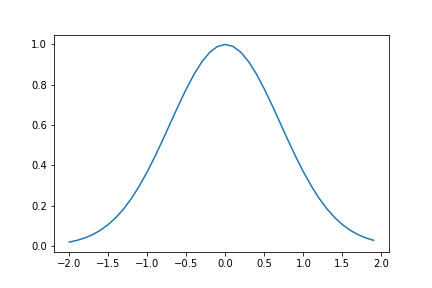
\includegraphics[width=120mm,bb=0 0 432 288]{../figures/normal2.png}
  \caption{式(\ref{eq:normal2})の図}
\end{figure}

この関数の説明はいりませんね? 指数関数の二乗の負版です.\\
まず, 世の中の多くの事象は平均値を取る確率が一番大きく, 平均値から離れるにつれその値を取る確率は小さくなることが知られています. んで, これをどう数式で表現すれば良いかと悩んだ末考えだされたのが正規分布関数だと思ってください.\\
 そうすると, とりあえず釣り鐘型の関数が欲しいという事で式(\ref{eq:normal2})を考えました. 実際これでほぼ完成です.\\
 ただ, これは任意定数がないため平均が0, 分散(幅)も一定ですね. これでは実用できません. そこで任意定数を導入し, 平均値と分散を可変にします. \\
 まずは平均値, つまりこのグラフの頂点の位置を動かします.\\

\begin{eqnarray}
\label{eq:normal3}
f(x) = e^{-(x-\mu)^2}
\end{eqnarray}

二次関数で高校の時にやりましたね.\\
\\
 次に, 分散...つまりこの釣り鐘の幅というか広がり方を変えます. \\

\begin{eqnarray}
\label{eq:normal4}
f(x) = e^{-\frac{(x-\mu)^2}{\sigma^2}}
\end{eqnarray}

平均に比べて一寸難解かもしれません. σ, つまり標準偏差で割る事で, σの値が小さければ鋭く, 大きければ扁平なグラフになります.\\
\\
 ただ, σは正負が定まらないため, 二乗して分散の形にする事で符号を一定にするわけです. \\
\\
 ともあれ ... これで, 母平均と母分散によって形を変える釣り鐘型分布が完成です!!めでたい!!\\

\begin{figure}[H]
\label{im:normal}
  \centering
  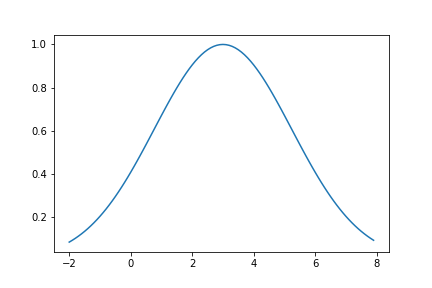
\includegraphics[width=120mm,bb=0 0 432 288]{../figures/normal4.png}
  \caption{式(\ref{eq:normal4})の図.(平均3, 分散10の場合)}
\end{figure}

え?式(\ref{eq:normal})と違うじゃないかって?\\
 せっかちだなぁ......余裕がない人間はモテないですよ.\\
\\
 まあ, グラフの形は実際これで完成なのです. ただ, 今我々が求めていたのは正規分布の「確率密度関数」でしたね?\\
\\
 確率の密度なのですから, 当然合計して1にならないといけないわけで, 先程の式(\ref{eq:normal4})ではその点がダメなのです. ちゃんと全確率点での値を足して1になるように正規化する必要があります.\\
\\
 つーわけで積分方程式を解きますがその前に, 出てくる計算結果を綺麗にするために式(\ref{eq:normal4})に細工をし, $\sigma^2$を$2\sigma^2$にしておきます. 2が付きましたが, グラフの性質自体は変わりませんね?\\
\\
 では積分方程式.
\begin{eqnarray}
\int_{-\infty}^{\infty} c e^{-\frac{(x-\mu)^2}{2\sigma^2}} dx= 1
\end{eqnarray}
を解きます...出来たものがこちらです.

\begin{eqnarray}
\label{eq:c}
c = \frac{1}{\sqrt{2\pi\sigma^2}}
\end{eqnarray}

式(\ref{eq:c})で得られたcを改めて式(\ref{eq:normal4}の変形版)に代入すると

\begin{eqnarray}
f(x) = \frac{1}{\sqrt{2\pi\sigma^2}}e^{-\frac{(x-\mu)^2}{2\sigma^2}}
\end{eqnarray}

が出てきましたね!良かった良かった. 以上が正規分布の確率密度関数の導出工程でした. フーリエなんかに比べれば雑魚ですね!ワンパンでした!\\
 え?積分方程式の解き方ですか?なんかMATLABにお願いしたら解いてくれました...

\subsubsection{100p\%点}
次. 正規分布を学ぶ意味は, この概念があるからといっても過言じゃない重要な性質です. 正規分布は平均が丁度真ん中で, 広がり方は分散によって定義される左右対称な特殊な分布でしたね?\\\\
つまり, 平均の周辺であるほど高確率で観測され, 裾野ほど「レア」な事象というわけです.\\\\
この性質を利用して, 正規分布には「100p\%点」と呼ばれる指標を導入する事が出来ます. これは「その点以上(以下)の部分の確率の合計がpになる境界」を指します. x軸の正方向なら上側, 負方向なら下側, 両方を指すなら両側100p\%点です. \\\\
言葉だとややこしいですが, グラフで見れば一瞬で分かります.


\begin{figure}[H]
\label{im:upper}
  \centering
  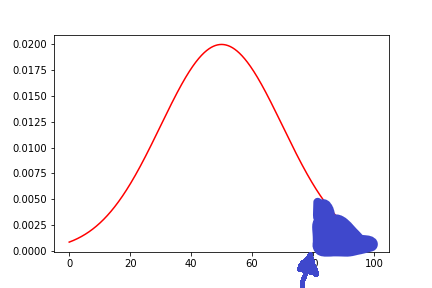
\includegraphics[width=120mm,bb=0 0 432 288]{../figures/upper_p.png}
  \caption{正規分布の上側5\%点}
\end{figure}

\begin{figure}[H]
\label{im:bilateral}
  \centering
  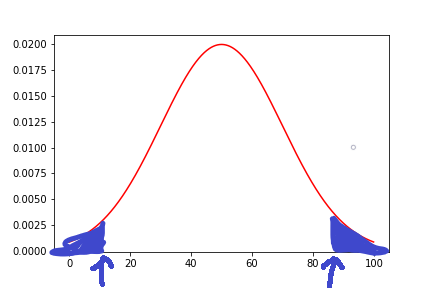
\includegraphics[width=120mm,bb=0 0 432 288]{../figures/bilateral_p.png}
  \caption{正規分布の両側5\%点}
\end{figure}

上側5\%に比べ, 両側5\%は左右に領域が分散した分上側の領域が狭くなってるのに注意です. \\
\\
だいたい, 正規分布でよく用いられるのは上下両側の5\%と1\%点です. 何に使うのかはあとで説明するので, ひとまず概念だけ覚えておいてください.

\subsection{t分布}
少ない標本数をもとに母分散がわかっていない母集団の母平均推定に使われるのがt分布です. 詳しくは推定の項で触れるので, ここでは確率密度関数と性質の確認をします.

\begin{eqnarray}
\label{eq:student}
f(x) = k(1 + \frac{x^2}{\alpha})^{-\frac{\alpha+1}{2}}
\end{eqnarray}

式(\ref{eq:student})がt分布の確率密度関数です. ここで$k$は定数, $\alpha$は自由度という指標で, この形を「自由度$\alpha$のt分布」と表現します. 自由度とは何かはここでは説明しませんが, 母集団によって算出できる値です. それ以外の部分では正規分布に似ていますね. 実際, 自由度$\alpha$が十分に大きい場合には正規分布になります. ただこいつの平均と分散は

\begin{eqnarray}
\mathbb{E}(X) = 0\\
\mathbb{V}(X) = \frac{\alpha}{\alpha-2}
\end{eqnarray}
です. 

\begin{figure}[H]
\label{im:student}
  \centering
  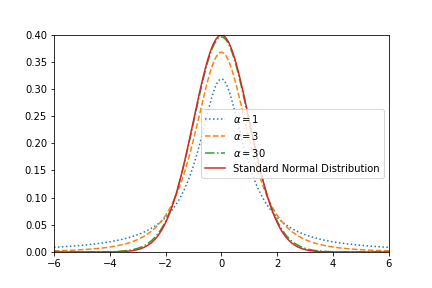
\includegraphics[width=120mm,bb=0 0 432 288]{../figures/student.png}
  \caption{自由度の異なるt分布と標準正規分布}
\end{figure}
自由度の異なるt分布と標準正規分布の比較です. 標準正規分布とは, 正規分布のうち平均が0, 分散が1のやつです. $\alpha$の値が大きいとほぼ同じ形になる事が分かると思います.\\
\\
では何に使うのかですが, そこはひとまず置いておきます. とにかくこういう分布があるのです.


\subsection{F分布}
F分布は, 少し特殊な形をしていますが非常に重要です. どう重要かというとF分布はこれまでの分布と異なり, 2つの母集団から得られた標本分散の比の確率分布になります. これの何がすごいのかというと, 例えば図(\ref{im:f_dist})は自由度が3の母集団Aと自由度が10の母集団BのF分布ですが, 「普通は」この組み合わせだと0から2あたりの値になる事が多いのです. \\
\\
しかしもし今, 自由度3と10のとある母集団A,B間でF値を取ったら6とかが出たとします. \\
通常はありえない値, つまり統計的に考えると「自由度だけでなく分散そのものに差がある = A,Bの母集団は異なる」となるわけですね. こちらも詳しくは後程. 式はえぐえぐです. 震えろ.

\begin{eqnarray}
f(x) = \frac{kx^{\frac{m}{2}-1}}{\{1 + (\frac{m}{n})x\}^{\frac{m+n}{2}}}
\end{eqnarray}

こいつの導出はいいです. 僕もわからん. 気が向いたら勉強してまとめるかも. 例によってkは定数, m,nは標本集団2つのそれぞれの自由度です. こいつは「自由度m,nのF分布」と表現されます. 今はそれだけ. 続いてグラフです. 幸いこっちは簡単.

\begin{figure}[H]
\label{im:f_dist}
  \centering
  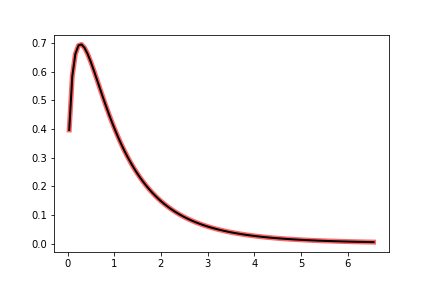
\includegraphics[width=120mm,bb=0 0 432 288]{../figures/f_dist.png}
  \caption{自由度3.10のF分布}
\end{figure}

恒例の平均値と分散です. こいつらも殺意高めだけど覚える必要は今のところ皆無だと思ってます.

\begin{eqnarray}
\mathbb{E}(X) = \frac{n}{n-2}\\
\mathbb{V}(X) = \frac{2n^2 (m+n-2)}{m(n-2)^2(n-4)}
\end{eqnarray}

\subsection{$\chi^2$分布}
ラスト. $\chi^2$分布です. こいつも重要です. 我々は結果を理論に落とし込む時, なんらかの数式に近似したり回帰したりするわけですが, 実際問題理論と観測値が完全に一致するなんていう事はまれで, 様々な要因で若干の誤差が生じます. その誤差が「誤差」なのか「理論の誤り」なのかを評価する時に使うのがこの分布とそれに基づく検定です. \\
\\
式はこちらです. 
\begin{eqnarray}
f(x) = k\chi^{\frac{\alpha}{2}-1}e^{-\frac{\chi}{2}}
\end{eqnarray}

またえぐえぐですね. えぐえぐと言えば, 筆者は声優の江口拓也さんが「やはり俺の青春ラブコメは間違っている」のラジオでやっていた「ぼっちラジオ」が大好きです. どうせこんな数学の同人誌読んでる人は陰キャだし, 楽しめると思います. 是非YouTubeで検索してみてください.\\
\\
さて, 例によってここの$\alpha$は自由度, kは定数です.\\
幸い, どこの説明を見てもこの式は使わないと言われているので覚えなくていいでしょう.\\
\\
平均値と分散です.
\begin{eqnarray}
\mathbb{E}(X) = \alpha \\
\mathbb{V}(X) = 2\alpha
\end{eqnarray}
簡単すぎワロタww\\
ついでグラフです.


\begin{figure}[H]
\label{im:chi}
  \centering
  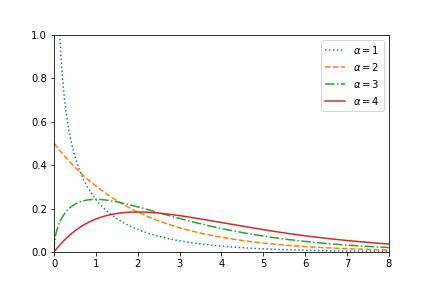
\includegraphics[width=120mm,bb=0 0 432 288]{../figures/kai.png}
  \caption{自由度の異なる$\chi^2$分布}
\end{figure}
 こいつは結構F分布に似てますね. ただ注意が必要なのは, F分布は標本分散の比に関する分布ですが$\chi^2$分布は標本分散そのものの分布です.

\newpage
\section{ベイズ統計}
\subsection{頻度主義とベイズ主義}
これに触れるのは気が引けるというか,ややこしいのですがどの統計本もこの話題から触っているので一応.確率を考える方法には,どうやら ``主義''があるようです.確率や統計はその性質上,絶対的な正解というものは存在しません.「こんな傾向があるよね」なんて議論を数学的にやろうという話なので,絶対はないからです.それ故,考え方の基礎というか根っこの部分で置く仮定のようなもので派閥が別れるのかななんて思っています.\\
 とかく,確率には頻度主義と呼ばれる派閥とベイズ主義と呼ばれる派閥があります.この派閥という表現だと対立しているようにも思えますし,実際対立している面倒な人達もいるようですが実際の現場ではどちらも便利なところがあるし,要は使い分けだと思います.よってどちらが優れているとか,どちらが正解とかいう議論は無意味だし,答えもないと思います.注意してください.\\
\\
 ということで,筆者はこうした宗教戦争には興味がないのと下手に触れると炎上しそうなので紹介だけです.興味があるようなら自分で勉強してみてください.正直自分はよく分かってないです.

\subsection{加法定理と乗法定理}
ベイズ統計に入る前に,確率に関する基本的な法則を二つ導入しておきます.加法定理と乗法定理です.三角関数とかでおなじみのあれです.確率の加法と乗法について考えてみましょう.\\
\\
 まずは加法定理から.確率変数$X,Y$を導入します.それぞれ$X=x_i, Y=y_j$を取る確率を$p(X=x_i, Y=y_j)$と書き,これを$X=x_i, Y=y_j$の同時確率と言います.\\
 ここまでは良いですよね.$x_iとy_j$が同時に観測される確率だから同時確率です.\\
\\
 さて,この$X, Y$の両方についてそれぞれサンプルを取る作業をN回行う事にします.この時,$X=x_i, Y=y_j$となる試行の回数を$n_{ij}$と表します.こうすると,以下の式が成り立ちますね.

\begin{eqnarray}
\label{eq:prob1}
p(X=x_i, Y=y_j) = \frac{n_{ij}}{N}
\end{eqnarray}

これは普通に,「大小のさいころ2つを振って大3,小6を引く確率(同時確率)を求めよ」とかと同じです.全試行分の当該試行ですね.
\\
 では次に,$X=x_i$となる確率を考えます.Yが取る値と関係なく,$X=x_i$となる試行数を$c_i$としておきましょう.そうすると,$p(X=x_i)$は

\begin{eqnarray}
\label{eq:prob2}
p(X=x_i) = \frac{c_i}{N}
\end{eqnarray}

になります.「大小2つのさいころを振って,大きい方が6になる確率は?」です.うーん?この例あまり良くないですね.どちらにせよ試行数1なので...まあいいや.\\
 この式(\ref{eq:prob2})ですが,式(\ref{eq:prob1})を使ってあえて複雑に書けばこうなります.

\begin{eqnarray}
\label{eq:sum-rule}
p(X=x_i) = \sum_{j=1} p(X=x_i, Y=y_j) = \sum_{j=1} \frac{n_{ij}}{N}
\end{eqnarray}

Yの値はなんでも良いから,Xが$x_i$になる確率を出したのが式(\ref{eq:prob2})なので,これは全ての$Y=y_j$について式(\ref{eq:prob1})を足し合わせたものと同じだよねという式になります.\\
\\
 これが確率の加法定理です.また,捉え方を変えるとこの処理はx以外の変数(ここではy)についての周辺化をするとも言い,式(\ref{eq:sum-rule})をxの周辺確率とも言います.\\
\\
 次に,$X=x_i$が既に観測されている状況に限って,その中で$Y=y_j$が観測される可能性を考えます.これを条件付き確率と言い,今の例だと以下のようになります.

\begin{eqnarray}
\label{eq:conditional}
p(Y=y_j | X=x_i) = \frac{n_{ij}}{c_i}
\end{eqnarray}

左辺の記法,最初は慣れないかもしれませんが慣れましょう.縦線は条件付きである事を表し,「右側の条件の元の左についての~~」を意味します.逆にならないように注意.筆者は最初よく逆に捉えていてわけわからんになっていましたが,これ以降頻繁に出てくる表現です.ここでは,上で述べたように ``$X=x_iの時のY=Y_iの確率(p)$''という意味です.\\
 式に戻りますが,右辺は分母に$X=x_i$になる試行数である$c_i$が来ていて,分子はXとYが$x_i, y_j$になる試行数である$n_{ij}$ですね.言葉の通り,$X=x_i$が確定した状況での$Y=y_j$が成り立つ可能性になっている事が分かるかと思います.\\
\\
 以上の事から確認されるように,加法定理同様,式(\ref{eq:prob1},\ref{eq:prob2})を考慮すると

\begin{eqnarray}
\label{eq:product}
p(X=x_i , Y=y_j) = p(Y=y_j | X=x_i)p(X=x_i)
\end{eqnarray}
が言えます.つまり,$X=x_i , Y=y_j$の同時確率は$X=x_i$が観測された上での$Y=y_j$の確率であり,これらの乗算によって求められるという事です.一応計算しても,

\begin{eqnarray}
\label{eq:product}
p(Y=y_j | X=x_i)p(X=x_i) = \frac{n_{ij}}{c_i}\frac{c_i}{N} = \frac{n_{ij}}{N}
\end{eqnarray}

で式(\ref{eq:prob1})が確かに求められていますね.これが確率の乗法定理です.意味するところは,$X=x_i, Y=y_j$の同時確率は$X=x_i$の確率と,$X=x_i$の元での$Y=y_j$の条件付確率との積である,ということになります.
\\
 まとめると,確率論の基本法則2つは以下になります.

\begin{screen}
確率の基本法則
\begin{eqnarray}
p(X) = \sum_Y p(X,Y) \qquad \text{加法定理} \nonumber \\
p(X,Y) = p(Y|X)p(X) \qquad \text{乗法定理} \nonumber
\end{eqnarray}
\end{screen}

ここでp(X)は確率変数Xの確率分布を指します.なので先程までの記法に従うと$p(X=x_1, x_2, x_3, ..., $となります.面倒なので以降はこうやって省略します.

\subsection{ベイズの定理}
いよいよベイズに行きます.ここではベイズ統計の歴史だとか主義がどうとかは一切触れないので,ぬるっと導入していきます.筆者がベイズいまいち分からん気がする理由は,ここでぬるっと導入できちゃうところにあったりもします.つまり主義がだの仮定がだの言っている割に,いわゆる頻度統計(?)で使ってる普通の式の変形でだせちゃうんですよね.いきます.\\
\\
 まず,同時確率は対称です.つまり$p(X,Y) = p(Y,X)$です.式(\ref{eq:prob1})より自明ですね.この性質を使って遊んでいるとベイズの定理が出てきちゃいます.

\begin{eqnarray}
\label{eq:bayes}
\begin{split}
p(X, Y) &= p(Y|X)p(X) \\
\therefore p(Y|X) &= \frac{p(X,Y)}{p(X)}  \\
\therefore p(Y|X) &= \frac{p(X|Y)p(Y)}{p(X)} \qquad \because p(X,Y) = p(Y, X)
\end{split}
\end{eqnarray}

できちゃいました.$\therefore, \because$の使い方あってるかな?あってるよね.$\therefore$はtexだとthereforeって書き,$\because$はbecauseって書きます.これで分かりますね?\\
\\
 さて,あっさりとベイズの定理が出せちゃったわけですが,その意味を解釈する前にもう一つ導きたい式があります.分母にいる$p(X)$に関して,加法定理と同時確率の対称性を使って

\begin{eqnarray}
\label{eq:bayes-x}
p(X) = \sum_Y p(X,Y) = \sum_Y p(Y,X) = \sum_Y p(X|Y)p(Y)
\end{eqnarray}
が言えますね.これを使って書き直した特殊な表現と原型を以下にまとめます.

\begin{screen}
ベイズの定理
\begin{eqnarray}
p(Y|X) &= \frac{p(X|Y)p(Y)}{p(X)}\\
p(Y|X) &= \frac{p(X|Y)p(Y)}{\sum_Y p(X|Y)p(Y)}
\end{eqnarray}
\end{screen}

上の式がよく見るベイズの形.下は式(\ref{eq:bayes-x})を使って定義しなおした式です.下を使って,ベイズの定理の意味するところを見ていきましょう.右辺の分母は,分子の計算を全てのYについて足し合わせたものになっています.つまりこれは,左辺の条件付確率を全てのYについて足し合わせると1になるように正規化しているのだという事がわかります.\\
 大小2つのさいころの例で考えるなら,こんな感じ


\begin{eqnarray}
\begin{split}
p(小=1|大=3) &= \frac{p(大=3|小=1)p(小=1)}{p(大=3|小=1)p(小=1) + ... + p(大=3|小=6)p(小=6))}\\
&= \frac{\frac{1}{6} \times \frac{1}{6}}{\frac{1}{36} + \frac{1}{36} + \frac{1}{36} + \frac{1}{36} + \frac{1}{36}+ \frac{1}{36}}\\
&= \frac{1}{6}
\end{split}
\end{eqnarray}

このことから,ベイズの定理の大事な部分は分母以外の$p(Y|X), p(X|Y),p(Y)$になります.こいつらについてそれぞれ何を意味しているのか考えていきましょう.\\
\\
 まず$p(Y)$と$p(Y|X)$です.$p(Y)$は単純ですね,確率変数Yの分布です.これは,計算を行う前から我々が「知っている」分布なので,Yの事前分布といいます.\\
 知っているとは何かというのがベイズ確率の面白い?批判されている?ところで,ここで置く分布はなんでもいいです.「さいころなんだから全部1/6の一様分布でしょ」としてもいいし,「さっきから3ばかり出てるから3が60\%くらいな気がする」でも,「3が全然出てこないからそろそろ出てきそう」でもいいし,とにかく,Xを観測する前に想定されているYの確率です.\\
\\
 一方,$p(Y|X)$は何かというと,Xを観測した元での,という条件付確率分布なので事後分布と呼びます.ベイズで求めるのは事後分布ですね.事前分布に何か($p(X|Y), p(X)$)をかけたり割ったりしてるので,事前分布を何らかの処理によって修正する過程とも捉えられることが分かります.\\
\\
\\
 残りは$p(X|Y)$ですね.こいつが多分一番納得しにくいのかなと思います.対称性使ってひょっこり持ってきた項だしね.これはXのYの元での条件付確率です.先程確認したように,ベイズの定理は事前確率$p(Y)$を,Xを観測した上での$p(Y|X)$に修正する過程でした.\\
 ここでYの元でのX,というのが何を指すかですが,事前確率Yの元でデータXが観測される可能性,ですね?言い換えると,「Yの値は$Y_j$である!」と仮定したときに$X_i$が得られる確率,となります.\\
\\
 なので,事前確率が正解に近いほど大きな値になり,逆に遠いほど小さい値になります.事前分布が,得られたXに対してどれだけもっともらしいのかを表すので尤度と呼ばれる量です.\\
\\
 以上を踏まえて,改めてベイズの定理を眺めると,正規化項を無視すれば

\begin{eqnarray}
事後分布 \propto 尤度 \times 事前分布
\end{eqnarray}

という式であると解釈する事ができます.\\
 事前分布で持ってきていた ``予想''の元で得られたデータがどれだけありえるかで予想を修正していくわけですね.あ,$\propto$は比例を意味する記号です.\\
 理解を深めてもらうため,一つちゃんとベイズっぽい例題を考えてみます.\\
\\
 研究室Aと研究室Bがあります.研究室Aは男4人,女6人,研究室Bは男8人女2人だとします.多分
 研究室Aは心理系のわりかしほんわかしたところで,研究室Bはくさいオタクが多そうですね.女性2人の心労はすごそうです.\\
 それはさておき,今ここからどちらかの研究室を選択し,無作為に3回授業の手伝いのために雑用を選んで来たら,男男女だったとします.さて,最初に選んだ研究室はどちらでしょう?という問題を考え,ベイズ的に解いてみましょう.\\
  \\
 研究室がA,Bである事象をそれぞれ$L=L_a, L_b$とし,選んだのが男女である事象を$S=S_m, S_f$
とします.\\
 今,1回目に男性が選択された時の研究室A,Bそれぞれの事後確率を計算してみましょう.ベイズの定理を使って表してみます.
  
\begin{eqnarray}
p(L_a | S_m) = \frac{p(S_m|L_a)p(L_a)}{\sum_L p(S|L)p(L)}\\
p(L_b | S_m) = \frac{p(S_m | L_b)p(L_b)}{\sum_L p(S|L)p(L)}
\end{eqnarray}

こうなりますね.次に各変数に実際の値を代入していきます.まず研究室の選択方法は無作為であったと仮定し,事前分布は一様,つまり$p(L_a)=p(L_b)=\frac{1}{2}$とします.$p(S_m|L_a), p(S_m|L_b), p(S_m)$は上記の設定より普通に計算できるので,1回目の試行での事後確率は以下のようになります.

\begin{eqnarray}
p(L_a | S_m) = \frac{\frac{4}{10} \times \frac{1}{2}}{ \frac{4}{10}\times \frac{1}{2} + \frac{8}{10}\times \frac{1}{2}} = \frac{1}{3}\\
p(L_b | S_m) = \frac{\frac{8}{10} \times \frac{1}{2}}{ \frac{4}{10}\times \frac{1}{2} + \frac{8}{10}\times \frac{1}{2}} = \frac{2}{3}
\end{eqnarray}

これはまあ普通ですよね.単純に全体のうち男性の比率が研究室AとBで1:2になっているのを反映しています.では次に2回目の試行について考慮します.1回目に男性が出たという事から,研究室AorBという事前分布が更新されます.\\
 先程は一様にどちらも50\%という仮定でしたが,今回は研究室Bである確率が高いと考えて事前分布を設定します.注意が必要なのは,分子の事前分布のみでなく分母に含まれている$p(Y)$の値もそれぞれ更新されている事です.この点,あえて$p(S_m)$と書かない今回の記法の方が理解しやすいと思います.

\begin{eqnarray}
p(L_a | S_m) = \frac{\frac{4}{10} \times \frac{1}{3}}{\frac{4}{10} \times \frac{1}{3} + \frac{8}{10} \times \frac{2}{3}} = \frac{1}{5}\\
p(L_b | S_m) = \frac{\frac{8}{10}\times \frac{2}{3}}{\frac{4}{10} \times \frac{1}{3} + \frac{8}{10} \times \frac{2}{3}} = \frac{4}{5}
\end{eqnarray}

確率が更新されました.これがベイズの「母数自体がパラメータ」という考え方を反映していて,唯一無二の確率を出すというよりも「今まで得られているデータからはこんな事が言えそう」という主張です.よってデータを得るたびに逐次的に更新する事が出来ます.\\
 これを使ったのが,後で触れる逐次学習だったりになりますがそれはとりあえず置いておきます.\\
 さて,最後.今まで男男と連続で引いたので,やはり男性率の圧倒的に高い研究室Bである確率が高いという事になっています.しかし最後は女性を引きます.どうなるでしょう?\\

\begin{eqnarray}
p(L_a | S_f) = \frac{\frac{6}{10} \times \frac{1}{5}}{\frac{6}{10} \times \frac{1}{5} + \frac{2}{10} \times \frac{4}{5}} = \frac{6}{14}\\
p(L_b | S_f) = \frac{\frac{2}{10}\times \frac{4}{5}}{\frac{6}{10} \times \frac{1}{5} + \frac{2}{10} \times \frac{4}{5}} = \frac{8}{14}
\end{eqnarray}

ありゃ,意外とがっつり削られたな.こんなもんなのか.3回目に女性を引いたことによって,今まで高まっていた研究室Bである確率ががくりと落ち,逆にAである確率が上がりましたね.とはいえまだBが優勢...という状況です.\\
 例のごとく事前分布$p(Y)$は更新されているので注意.ベイズ統計はこのようにして予想を適宜修正していくような使い方が出来るわけですね.この,少しずつ分布を更新していく過程をベイズ更新とも言います.これゆえ機械学習だとか脳のモデルと相性が良いわけです.つまり,得られたデータを毎瞬反映させて少しずつ内部モデルを更新していけるわけです.つよい.\\
\\
 面倒なので計算はしませんが,一つ皆さんも気になるだろう話題について問題提起だけしておきます.今回の問題では研究室AかBのどちらが選ばれたのか最初に一様分布を仮定しましたが,そうじゃない場合はどうなるでしょう?\\
 雑用を選ぶ問題だったので,なんとなく先生の力が弱い方の研究室が押し付けられそうですよね.研究室Aは新任の特任准教授,研究室Bは学部長の主催するラボだったとしましょう.そうするとなんとなく,押し付けらそうなので事前分布に研究室A75\%, Bが25\%とかって仮定をおいてみたくなります.\\
\\
 アカデミア,政治色強いですよね.研究は大した事なくても政治だけでのしあがっていく先生も多いし,闇を感じるところは多々あります.いや,筆者もおそらく政治強い側の人間になりそうなので強く言えませんが...コネって大事ですよね.\\
\\
 閑話休題.
\\
\\
 さて,暇な人はこのように事前分布を変えて計算してみてください.当然結果は変わります.そしてこの点がまさに,ベイズに批判的な人達の武器で,事前分布に何を用いるかが結局強く影響しちゃうんですよね.なのでベイズを用いる際は,事前分布の妥当性はちゃんと検証しなければならないです.

\subsection{ベイズの応用}
応用,というか実際にベイズを何にどうやって使っていくのかという話です.まず,ここまでベイズは離散で考えてきましたが当然連続確率分布でも計算できます.むしろそっちの利用の方が多いでしょう.まぁ例のごとく基本は$\sum$を$\int$に変えるだけです.\\
 これを使ってどんなアプリケーションが使えるのかというと,先程の逐次学習がまずあります.次々観測されるデータを元に,内部モデルを更新していく過程ですね.パターン認識,機械学習,それから脳のモデルなんかに頻繁に適用されて議論されます.\\
\\
 自分の専門でもあるから少し述べるなら,脳は常に環境に適用するため,次に何が起きるのかや,得られた刺激がどういったものなのかを推定していく必要があります.\\
 同時に,もしその推定が間違っているなら修正していく必要があるし,うまくいったなら強化していくと嬉しい事がありそうです.まさにこの過程がベイズ使った更新なんじゃない?みたいな話になっていくわけですね.\\
\\
 まぁ実際はそんな単純じゃないし,上に書いたような内容はひどく古いというか単純な話です.もう少し複雑だったり,厳密にはちょっと違ったりしてきます.がこれ以降は万人に共通して必要な知識というほどでもないと思うのでadvancedの方に引き渡します.興味ある人は読んでみてください.
\section{統計的推定}
なぜ確率分布のあとにベイズに突然触れたかというと,この章で扱う推定に密接に関わってくるからです.実世界で統計を使っていく上で重要なのは,あるデータ群が形成する分布の種類を特定する事ではありません.ただ分布型が分かっただけでは大抵,なんの役にも立ちません.\\
 重要なのは,その分布の平均や分散です.クラスのテスト成績が正規分布に従う事を知っていても,肝心の平均点などが分からないと学生は喜んでいいのか落ち込むべきなのか分からないし,教員も授業内容の補修をするべきかもっと踏み込んだ議論をするべきか分かりません.\\
\\
 という事で,母集団の確率分布を規定する ``母数''を推定したくなります.母数は,たとえば母平均や母分散といった量があります.母平均の推定はわりとよくやっていますね.\\
 あるクラスでてきとうに選んだ5人の点数$(X_1,X_2...X_5)$があれば,彼らの平均からクラス全体の平均を推定しようとするでしょう.これが母数の推定です.\\

\begin{eqnarray}
\label{eq:est1}
\hat \mu = (X_1 + X_2 + ... X_5)/5
\end{eqnarray}

この式では,母平均$(\mu)$の推定を行っています.$\mu$の上についている $\hat \mu$ は推定値である事を意味します.当然,母集団全てを加算平均してだした $\hat \mu$ は $\mu$と同じ値になります.しかし現実には母集団全てを観測し計算するなど不可能なことが多いため,その一部のみを使ってうまく母数に近づけた推定値を求めていく必要があります.\\
\\
 あるいは,統計的ないわゆる○○分布ではないけれどもなんらかの関数で説明できるような変化,分布も多くあります.これらを説明する際に,多項式曲線を使ってフィッティングしていったりするのですが,この際にもやはりこのモデルの形を定めるパラメータの適切な値を推定したくなります.\\
 こうした量を推定していく方法を勉強していきましょう.\\

\subsection{点推定と区間推定}
母数の推定値を求める際に,方法が大きく分けて2種類あります.それが点推定と区間推定です.簡単ですが一応.点推定は先程の式(\ref{eq:est1})のように母数をある一つの値 $\hat \theta$ で指定する方法を指します.なおここで$\theta$は母数を表す一般化記号で,実際には$\mu, \sigma$などがあてはまります.\\
\\
 単一の点で推定をする以上,どうしても実際の母数との誤差が生じます.そのため,この誤差を最小化していきたいというのが点推定の主なモチベーションです.\\
\\
 区間推定は,点推定と異なり推定に幅を持たせる方法です.たとえば,A組のテストの平均点は50-60点の間である.などといった推定です.

\subsection{最尤推定}
まずは点推定のうち,頻度主義でよく使われる最尤推定を考えます.そのために,まずはベイズの時に出てきていた尤度についてもう少し考えます.尤度は何もベイズ主義の用語ではありません.頻度主義でもよく使うもので,結局ベイズと頻度とのちがいは何かというと事前分布を用いるかの方にあります.\\
 で,尤度ですが,事前確率を評価しているという風に言っていましたが推定の枠組みで考え直します.推定は分布の母数だったり,あるいはより複雑な多項式曲線フィッティングだったりするので,こいつらを確率変数ベクトル$\mathbf{w}$とします.たとえば$\mathbf{w} = [\mu, \quad \sigma]$とかです.\\
\\
 観測データをDでおくと,ベイズの定理は以下の形を取ります.

\begin{eqnarray}
p(\mathbf{w}|D) = \frac{p(D|\mathbf{w})p(\mathbf{w})}{p(D)}
\end{eqnarray}

ここで,尤度$p(D|\mathbf{w})$について考えるとデータ集合Dに対するベクトル$\mathbf{w}$による評価関数と捉えられます.事前分布を更新するという話の時と同様です.例のごとくp(D)は正規化しているだけなのでどうでもいいです.\\
\\
 さて,最尤推定ですが,読んで字のごとく尤度を最適化する推定方法です.尤度はパラメータベクトルの元での,得られたデータの尤もらしさを評価する関数なので,これを最大化する事で最も尤もらしいパラメータの推定値,最尤推定値を求める手法です.実際に例を考えながら説明してみます.\\
\\
 ある研究室(A)に所属する学振特別研究員の数を推定したいとします.学生(S)の数は5人にしておきましょう.推定したいパラメータ(DC研究員数)をiとします.そうすると
\begin{eqnarray}
p(S=DC | L) = \frac{i}{5}
p(S=凡人|L) = \frac{5-i}{5}
\end{eqnarray}
と尤度を仮定できます.最尤推定の基本は,尤度が最大の事象が観測されたという仮定を置くことにあります.よって,観測された事象分の尤度をかけ合わせて,最大になるパラメータiの値を採用します.\\
\\
 たとえば今回,研究室Aから適当に人を選んできてDCに採用されているか確認したところ,採用採用不採用となっていたとします.その場合尤度関数L(S; i)は
\begin{eqnarray}
L(S; i) = \frac{i}{5}^2 \frac{5-i}{5}
\end{eqnarray}
 となります.こいつを最大化すれば良いわけですね.ちなみに記法ですが,f(x;y)という記法は数学ではパラメータyによって規定される変数xの関数,という意味です.ここではyは変数ではなく,fを定義する際の固定値になります.だからこそ,今回は固定値として使うiの値を最適化したいというモチベになります.\\
 せっかくなんで手計算.\\

\begin{eqnarray}
L(S;i) \propto -i^3 + 5i^2\\
\therefore  L(S;i)' \propto i(-3i+10)\\
i = \frac{10}{3}
\end{eqnarray}

最大化は微分して0になる点を探せば良いんでしたね.今回のだとだいたい3が尤度最大の点でした.研究室AのDC学生は5人中3人であるという推定になります.優秀や...\\
\\
 なお,今回は大した計算じゃなかったのでそのままやりましたが実際は100試行とかになると尤度を掛け算でだすと値がすごい事になってしまうので対数に変換した対数尤度関数の最大化を行う事が多いです.対数に変換した場合,掛け算は足し算になるので計算が楽ですね.\\
\\
 さて,計算方法と気持ちが分かったところで以上の手順を一般化します.まずは尤度関数の定義から.

\begin{screen}
尤度関数
\begin{eqnarray}
L(\theta) = \Pi_{i=1} ^n f(x_i;\theta) \qquad \text{尤度関数}\\
logL(\theta) = \sum_{i=1}^n f(x_i;\theta) \qquad \text{対数尤度関数}
\end{eqnarray}
\end{screen}

大丈夫でしょうか.尤度関数のかけざんを対数尤度関数では足し算に変換しました.ここで$\theta$は母数だったり,とにかくパラメータです.パラメータ$\theta$によって規定され,変数xを変数とする尤度を全てのxについてかけあわせたのが尤度関数でした.\\
 対数尤度は計算を簡単にするため,それを対数変換したものですね.\\
\\
 で,最尤推定はこいつらを最大化する処理なので,最尤推定値$\hat\theta$は

\begin{eqnarray}
\label{eq:ML}
\hat\theta = \max_\theta L(\theta) = \max_\theta logL(\theta)
\end{eqnarray}


 となる$\theta$になります.記法ですが,$\max_\theta f(x;\theta)$はf(x)を最大化する$\theta$という意味です.\\
\\
\\
 余談ですが,対数尤度関数は最大化する事で尤もらしい値をだすものでしたが,機械学習とかだとよくこれを符号反転させた$-logL(\theta)$を誤差関数と呼び,これを最小化する方向にフィッティングしているようです.単調減少していくので,0に近付けるという意味で扱いやすいんでしょうね.







\subsection{ベイズ推定}
しかし本当に尤度最大化で良いのでしょうか?\\
 さっきの例だと,自分のラボを優秀に見せようとしたPIがわざと採択されている学生だけ選ばれるように仕向けていたのかもしれません.本当は1人しかいないかもしれないし,極端な話2回目の試行で止めていたら採用採用だったので採用率100\%,最尤推定の結果は当然,採択者5/5名となってしまいます.\\
\\
 これでは困りますよね.このように,最尤推定の弱点として十分な試行回数がないと極端すぎる結果を招きかねません.どうにか,尤度だけじゃなくて「あの教授は信用ならないしなぁ」とかといった事も考慮できないのでしょうか...\\
 え?なに?ベイズですか...?米ズ...米津......ベイズですね!!!!\\
 ベイズは尤度だけじゃなく,われらが奥義,事前分布がありました!これを使えば良いわけですね!!\\
\\
 という事で,最尤推定と同じ問題に取り組むもう一つの方法として,ベイズ推定があります.
\section{統計的検定}
\end{document}